% =============================================================================
% SAGE: Safe Architecture Graph Editing for Agentic Vulnerability Discovery
% via Constrained POMDPs
% ACM CCS 2026
% =============================================================================
\documentclass[sigconf,anonymous]{acmart}
\settopmatter{printacmref=false,printfolios=true}
    
% Package imports
\usepackage{nicefrac}
\usepackage{siunitx}
\usepackage{array,framed}
\usepackage{booktabs}
\usepackage{color,float,epsfig,wrapfig,graphics,graphicx,subcaption}
\usepackage{textcomp}
\usepackage{setspace}
\usepackage{latexsym,fancyhdr,url}
\usepackage{enumerate}
\usepackage{algorithm}
\usepackage{algorithmic}
\usepackage{xparse}
\usepackage{xspace}
\usepackage{multirow}
\usepackage{balance}
\usepackage{tikz}
\usepackage{pgfplots}
\usepackage{pgfplotstable}
\usepackage{hyperref}
\usepackage{mathtools}

\usetikzlibrary{shapes.geometric,arrows,positioning,fit,backgrounds,matrix,calc}
\pgfplotsset{compat=1.17}

% Custom commands
\DeclarePairedDelimiter\abs{\lvert}{\rvert}
\DeclareMathAlphabet{\mathcal}{OMS}{cmsy}{m}{n}
\newcommand{\E}{\mathbb{E}}
\newcommand{\R}{\mathbb{R}}
\newcommand{\ie}{\emph{i.e.}\xspace}
\newcommand{\eg}{\emph{e.g.}\xspace}
\newcommand{\etal}{\emph{et~al.}\xspace}
\newcommand{\SAGE}{\textsc{Sage}\xspace}
\newcommand{\secref}[1]{Section~\ref{#1}}
\newcommand{\figref}[1]{Figure~\ref{#1}}
\newcommand{\tabref}[1]{Table~\ref{#1}}
\newcommand{\eqnref}[1]{Equation~(\ref{#1})}
\newcommand{\algref}[1]{Algorithm~\ref{#1}}

\setlength{\belowcaptionskip}{-8pt}
\setlength{\abovecaptionskip}{5pt plus 3pt minus 2pt} 

% =============================================================================
\begin{document}

\title{SAGE: Safe Architecture Graph Editing for Agentic Vulnerability Discovery via Constrained POMDPs}

\author{Anonymous Authors}
\affiliation{\institution{Anonymous Institution}}

\begin{abstract}
Agentic security systems---compositions of language models with tools such as static analyzers, fuzzers, exploit validators, and patch generators---are increasingly deployed for automated vulnerability discovery. In practice, performance depends critically on architecture: which components exist, how they connect, and what model variants each uses. The optimal architecture is target-dependent, only partially observable during an engagement, and subject to change as both the target and security landscape evolve. Two constraints are unavoidable: budgets on computational resources, and safety requirements that prevent prompt-injection-driven tool misuse.

We introduce \SAGE, a framework for online architecture adaptation of agentic security systems. We formalize adaptation as a Constrained Partially Observable Markov Decision Process where the state includes the agent-tool graph, trace-derived features, and budget-risk meters, while actions correspond to reversible graph edits: adding or removing nodes, rewiring edges, adjusting parameters, and switching model variants. Safety is enforced through two layers: hard structural constraints via projection into an allowed-architecture set mandating guards between untrusted inputs and sensitive tools, and soft risk constraints via Constrained MDP optimization with Lagrangian updates.

We contribute: (1)~a formal C-POMDP specification of architecture adaptation with typed graph actions; (2)~a two-layer safety architecture separating structural invariants from risk budgets; (3)~learning algorithms from constrained contextual bandits to full constrained RL; and (4)~a reproducible synthetic case study where safe adaptive policies achieve $9.6\times$ higher reward than the best static safe architecture while maintaining zero constraint violations. We specify an evaluation protocol for security benchmarks and discuss limitations and responsible deployment.
\end{abstract}

\begin{CCSXML}
<ccs2012>
<concept>
<concept_id>10002978.10002991</concept_id>
<concept_desc>Security and privacy~Software security engineering</concept_desc>
<concept_significance>500</concept_significance>
</concept>
<concept>
<concept_id>10010147.10010257</concept_id>
<concept_desc>Computing methodologies~Reinforcement learning</concept_desc>
<concept_significance>500</concept_significance>
</concept>
<concept>
<concept_id>10010147.10010257.10010293</concept_id>
<concept_desc>Computing methodologies~Planning under uncertainty</concept_desc>
<concept_significance>300</concept_significance>
</concept>
</ccs2012>
\end{CCSXML}

\ccsdesc[500]{Security and privacy~Software security engineering}
\ccsdesc[500]{Computing methodologies~Reinforcement learning}
\ccsdesc[300]{Computing methodologies~Planning under uncertainty}

\keywords{Agentic security, architecture adaptation, constrained reinforcement learning, contextual bandits, prompt injection, tool misuse prevention, vulnerability discovery}

\maketitle

% =============================================================================
% SECTION 1: INTRODUCTION
% =============================================================================
\section{Introduction}
\label{sec:intro}

Security automation has entered a fundamentally new era. What once consisted of a scanner producing a static report has evolved into \emph{agentic workflows}: directed graphs of specialized components---large language models, static analyzers, fuzzers, exploit validators, patch generators, evidence stores, and policy guards---that interact through tool calls and structured memory. Frameworks for tool-using and multi-agent composition such as ReAct~\cite{yao2023react}, Toolformer~\cite{schick2023toolformer}, and AutoGen~\cite{wu2023autogen} have accelerated this trend in general-purpose AI applications. Security-specific systems such as PentestGPT~\cite{deng2024pentestgpt} demonstrate that decomposing penetration testing into interacting modules can help maintain context and improve task completion relative to monolithic prompting strategies.

A central observation motivates this work: \emph{architecture is destiny}. Two systems using the same underlying language model can produce radically different outcomes depending on how components are routed, how memory is scoped, where guards are placed, which model or tool variant is selected for each subtask, and when the system decides to probe versus patch. Consider a concrete scenario: an agentic system performing vulnerability discovery against a web application. Early in the engagement, broad reconnaissance with lightweight models maximizes coverage per dollar spent. As promising attack vectors emerge, the system benefits from switching to more capable models for precise validation. If the target begins exhibiting signs of prompt injection attempts in its responses, inserting additional guards becomes critical. A static architecture cannot respond to these dynamics; it must be designed conservatively enough to handle the worst case, sacrificing efficiency in typical cases.

This architecture adaptation problem exhibits three challenging properties. First, targets are only \emph{partially observable}: one never truly sees the complete state of the system under test, only the outputs of probes and tools. Second, the environment is \emph{nonstationary}: defenses change, software builds roll forward, rate limits activate, and adversaries may attempt to poison prompts. Third, two constraints are \emph{unavoidable}: budgets on computational resources such as tokens and wall-clock time, and safety requirements that prevent prompt-injection-driven tool misuse, data exfiltration, and policy violations.

A naive response to this complexity is to hand-design a single ``best'' architecture and hope it generalizes across targets and engagement phases. Empirically, this approach proves brittle even in adjacent domains such as software engineering agents, where interface design and tool access can dominate outcomes~\cite{yang2024sweagent}. In security applications, brittleness is amplified by adversarial inputs. Prompt injection in LLM-integrated applications has been demonstrated repeatedly in both research settings and production systems~\cite{liu2024promptinjection,greshake2023indirect}, and the OWASP Top~$10$ for LLM Applications explicitly lists prompt injection and insecure output handling among the leading risks~\cite{owasp2023llmtop10}.

This paper addresses a specific question:
\begin{quote}
\emph{How can an agentic security system adapt its own architecture online to maximize security utility under budget and safety constraints, when rewards are only revealed after execution?}
\end{quote}

The key insight is that architecture decisions---which components to include, how to wire them together, and which variants to deploy---can themselves be treated as \emph{actions} in a sequential decision problem. Crucially, \SAGE operates \emph{during} a security engagement, not just at design time: the system continuously monitors execution traces and adapts its architecture in response to observed conditions such as coverage plateaus, validation failures, or prompt injection alerts. By formalizing this problem as a Constrained Partially Observable Markov Decision Process and developing algorithms that learn from execution traces while respecting hard structural constraints and soft risk budgets, we can build systems that are both more effective and more trustworthy than fixed architectures.

\subsection{Contributions}

This paper makes the following contributions:

\begin{enumerate}
\item \textbf{Formal specification} (\secref{sec:problem}--\ref{sec:adaptation}): We define the Adaptation C-POMDP, a constrained partially observable control problem where states encompass agent-tool graphs, trace features, and budget-risk meters; actions are typed graph edits; and objectives trade off security utility against cost and risk constraints.

\item \textbf{Two-layer safety architecture} (\secref{sec:safety}): We introduce a design that separates hard structural constraints---enforced by projection into an admissible architecture set---from soft risk constraints enforced through Lagrangian optimization. Hard constraints guarantee that certain unsafe configurations are never instantiated; soft constraints bound expected cumulative risk within configurable budgets.

\item \textbf{Learning algorithms} (\secref{sec:learning}): We develop algorithms spanning constrained contextual bandits for stage-wise decisions to full constrained RL for continuous adaptation, with offline training and off-policy evaluation via doubly-robust estimators~\cite{jiang2016doublyrobust}.

\item \textbf{Empirical validation} (\secref{sec:casestudy}): We present a reproducible synthetic case study where a safe adaptive policy achieves $9.6\times$ higher reward than the best static safe architecture while maintaining zero constraint violations. We include ablation studies showing that both hard and soft constraints are necessary, sensitivity analysis across risk budgets, and learning dynamics characterization.

\item \textbf{Evaluation protocol} (\secref{sec:evaluation}): We specify benchmarks, baselines, and metrics for rigorous evaluation of architecture adaptation in security contexts.
\end{enumerate}

The remainder of the paper is organized as follows. \secref{sec:background} reviews background and related work. \secref{sec:problem} defines the problem setting and threat model. \secref{sec:adaptation} formalizes the Adaptation C-POMDP. \secref{sec:safety} presents the safety layer. \secref{sec:learning} develops learning algorithms. \secref{sec:system} describes system design. \secref{sec:evaluation} specifies the evaluation methodology. \secref{sec:casestudy} presents the synthetic case study. \secref{sec:discussion} discusses practical considerations and limitations. \secref{sec:related} surveys related work. \secref{sec:conclusion} concludes.

% =============================================================================
% SECTION 2: BACKGROUND AND RELATED WORK
% =============================================================================
\section{Background and Related Work}
\label{sec:background}

This section reviews the technical foundations and prior work that motivate and inform \SAGE. We organize the discussion around three themes: tool-using and agentic language models, security threats arising from prompt injection and tool misuse, and constrained decision-making frameworks from reinforcement learning.

\subsection{Tool-Using and Agentic Language Models}

Modern agentic systems interleave natural language reasoning with tool calls to interact with external environments. The ReAct framework~\cite{yao2023react} formalizes this pattern as alternating reasoning traces that articulate the agent's plan and actions that query the environment, demonstrating that explicit reasoning improves task completion on knowledge-intensive and interactive benchmarks. Toolformer~\cite{schick2023toolformer} shows how language models can learn to decide when and how to call tools by training on self-generated examples of useful tool invocations, enabling models to augment their capabilities with calculators, search engines, and translation services without task-specific fine-tuning. AutoGen~\cite{wu2023autogen} provides a general framework for multi-agent conversation patterns in which different agents specialize in different subtasks and coordinate through structured message passing.

These ideas map naturally onto security workflows where tools such as static analyzers, fuzzers, debuggers, and network scanners are core primitives. PentestGPT~\cite{deng2024pentestgpt} demonstrates that decomposing penetration testing into interacting modules---a reasoning module that maintains engagement context, a generation module that produces commands, and a parsing module that interprets tool outputs---can mitigate context loss and improve completion rates on penetration testing tasks relative to monolithic prompting. The architecture of such systems is not merely an implementation detail but a first-class design choice that affects capabilities, efficiency, and safety.

A growing body of work studies how to evaluate and improve the tool-using capabilities of language models. ToolLLM~\cite{qin2023toolllm} introduces a benchmark of $16{,}000$ real-world APIs and shows that fine-tuning on tool-use data substantially improves API calling accuracy. ToolAlpaca~\cite{tang2023toolalpaca} generates $3{,}000$ simulated tool-use cases to study generalization across tool categories. These benchmarks establish that tool selection and sequencing are learnable skills, motivating the idea that architecture-level decisions can similarly be optimized.

\subsection{Security Threats: Prompt Injection and Tool Misuse}

When an agent consumes untrusted text---web pages, log files, issue reports, crash traces, or outputs from other agents---prompt injection attacks can redirect tool usage, exfiltrate secrets, or cause policy violations. Liu~\etal~\cite{liu2024promptinjection} provide a large-scale empirical study demonstrating widespread vulnerability to prompt injection in real LLM-integrated applications, including systems that expose file system access, code execution, and network capabilities. Greshake~\etal~\cite{greshake2023indirect} introduce indirect prompt injection, in which adversarial instructions are embedded in content the agent retrieves rather than in the user's direct input, and show that this attack vector compromises multiple production systems including email assistants and code completion tools.

The OWASP Top $10$ for Large Language Model Applications~\cite{owasp2023llmtop10} codifies these risks for practitioners, listing prompt injection as the top threat and identifying related failure modes including insecure output handling, excessive agency, and over-reliance on model outputs. These taxonomies underscore that security in agentic systems is not merely an alignment problem to be solved through model training but also an architecture problem: where guards are placed, which tools are reachable from which components, and how untrusted inputs flow through the system all affect the attack surface.

Defense mechanisms have been proposed at multiple layers. Classifier-based prompt guards attempt to detect injection attempts before they reach the model, with recent work such as PIGuard~\cite{li2024piguard} and InjecGuard~\cite{injecguard2024} explicitly managing the tradeoff between detection accuracy and over-defense that causes legitimate queries to be rejected. However, no single defense is sufficient, especially when the system has powerful tools behind it. This motivates \SAGE's focus on architectural constraints as a first-class control object: even if prompt injection succeeds at one layer, structural guarantees can limit the blast radius.

\subsection{Constrained Decision Making}

Constrained Markov Decision Processes provide a principled framework for optimization with explicit costs or risks~\cite{altman1999cmdp}. The standard formulation seeks a policy that maximizes expected cumulative reward subject to constraints on expected cumulative costs. Constrained Policy Optimization~\cite{achiam2017cpo} provides a practical algorithm for this setting, using trust-region updates that guarantee approximate constraint satisfaction during learning. Subsequent work develops primal-dual methods that achieve last-iterate convergence~\cite{ding2024lastiterateconvergence} and extend to state-wise constraints where safety must hold at every step rather than only in expectation~\cite{zhao2023saferlsurvey}.

Surveys of safe reinforcement learning~\cite{kushwaha2024saferl,zhao2023saferlsurvey} summarize the landscape of techniques including Lagrangian methods, barrier functions, projection-based approaches, and constrained policy search. \SAGE applies these principles not to robot torque limits or collision avoidance but to security risk budgets and compliance constraints in a tool-using agent graph, requiring adaptation of the standard frameworks to handle the structure of graph-valued actions and the partial observability inherent in security engagements.

\subsection{Architecture Optimization}

The idea that architecture can be optimized rather than hand-designed has been explored extensively in neural architecture search. Zoph and Le~\cite{zoph2017nas} show that reinforcement learning can discover competitive neural network architectures by treating layer specifications as actions and validation accuracy as reward. While the action space and constraints differ substantially from \SAGE---neural architecture search optimizes static computational graphs for a fixed task, while we optimize dynamic agent graphs that must adapt during deployment---the conceptual precedent establishes that RL can handle structured, combinatorial action spaces.

In the multi-agent systems literature, work on learning communication protocols~\cite{lowe2017marl} and agent role assignment demonstrates that the structure of multi-agent interaction can be learned from data. Cognitive architectures for language agents~\cite{sumers2024cognitive} provide frameworks for reasoning about memory, planning, and tool use that inform how we structure the nodes and edges of agent graphs. Surveys of LLM-based autonomous agents~\cite{wang2024survey,xi2023rise} catalog the design patterns that emerge in practice, providing empirical grounding for the action space we consider.

\subsection{Positioning of This Work}

\SAGE differs from prior work in several key respects. Unlike static agentic systems such as ReAct or PentestGPT, \SAGE treats architecture as a dynamic control variable adapted online based on engagement feedback. Unlike neural architecture search, which optimizes the internal structure of neural networks (layers, connections, activation functions), \SAGE optimizes the \emph{multi-agent graph topology}: which agent and tool components exist, how they are connected, and what variants are selected---without modifying the internal neural networks of individual agents. Furthermore, \SAGE operates in a nonstationary, partially observable setting with explicit safety constraints, whereas NAS typically assumes a fixed task and offline optimization. Unlike general safe RL work, \SAGE addresses the specific structure of agent graphs with typed nodes and edges, projection-based hard constraints, and security-relevant risk metrics. The combination of these elements---online adaptation of multi-agent topology, safety constraints, and graph-structured actions in a security context---represents the novel contribution of this work.

% =============================================================================
% SECTION 3: PROBLEM SETTING
% =============================================================================
\section{Problem Setting}
\label{sec:problem}

\begin{figure}[t]
\centering
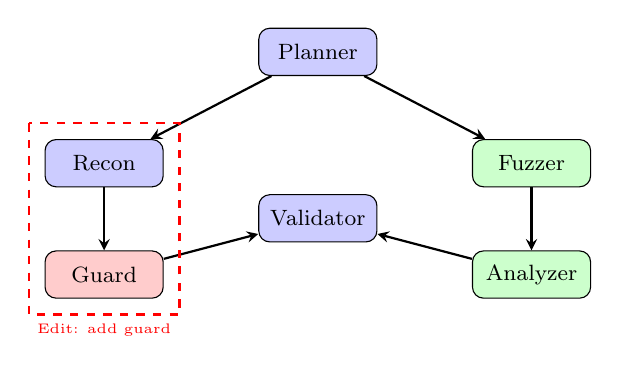
\begin{tikzpicture}[
    node distance=0.8cm and 1.2cm,
    box/.style={rectangle, draw, rounded corners, minimum width=1.5cm, minimum height=0.6cm, font=\footnotesize},
    guard/.style={box, fill=red!20},
    agent/.style={box, fill=blue!20},
    tool/.style={box, fill=green!20},
    arrow/.style={->, >=stealth, thick}
]
% Nodes
\node[agent] (planner) {Planner};
\node[agent, below left=of planner] (recon) {Recon};
\node[tool, below right=of planner] (fuzzer) {Fuzzer};
\node[guard, below=of recon] (guard1) {Guard};
\node[tool, below=of fuzzer] (analyzer) {Analyzer};
\node[agent, below=1.5cm of planner] (validator) {Validator};

% Edges
\draw[arrow] (planner) -- (recon);
\draw[arrow] (planner) -- (fuzzer);
\draw[arrow] (recon) -- (guard1);
\draw[arrow] (guard1) -- (validator);
\draw[arrow] (fuzzer) -- (analyzer);
\draw[arrow] (analyzer) -- (validator);

% Adaptation annotation
\draw[dashed, thick, red] ($(recon.north west)+(-0.2,0.2)$) rectangle ($(guard1.south east)+(0.2,-0.2)$);
\node[font=\tiny, red] at ($(guard1.south)+(0,-0.4)$) {Edit: add guard};
\end{tikzpicture}
\caption{Example agent graph with a guard node inserted on the path from reconnaissance to validation. \SAGE treats such architectural changes as actions in a sequential decision problem, learning when to add guards, switch components, or rewire edges based on engagement feedback.}
\label{fig:architecture}
\end{figure}

We consider an agentic security system operating against an authorized target, which may be a sandboxed benchmark, a capture-the-flag instance, or a legally scoped internal environment. The system's task is to discover vulnerabilities, validate exploits, and in some cases generate patches, all while respecting budget constraints on resources such as tokens and wall-clock time, and safety constraints that prevent unintended harm.

\subsection{Threat Model}

We assume a threat model appropriate for defensive security testing where the operator is authorized but the target may contain adversarial content. The operator controls the agentic system and defines its budget and risk constraints. The target system may be malicious or compromised, and may attempt to influence the agent through prompt injection embedded in application outputs, error messages, or data retrieved during reconnaissance. External data sources accessed during the engagement, such as documentation or issue trackers, may also contain adversarial content.

The attacker's goal is to cause the agent to misuse its tools in ways that violate the operator's intent: exfiltrating sensitive data, executing unauthorized commands, persisting malicious state that affects future sessions, or exhausting budget on attacker-chosen tasks. The defender's goal is to maximize security utility, measured by validated vulnerability findings or successful patches, while preventing these violations.

We do \emph{not} assume that prompt injection can be perfectly detected or prevented. Instead, we assume that architectural constraints can limit the consequences of successful injection, and that risk can be estimated from observable signals such as guard alerts and anomalous tool usage patterns. This defense-in-depth posture motivates the two-layer safety design introduced in \secref{sec:safety}.

\subsection{Environment and Architecture Graph}

The environment $\mathcal{E}$ encompasses the target system under test, the toolchain available to the agent, and monitoring infrastructure. The environment evolves stochastically over time as the target responds to probes, defenses adapt, rate limits activate, and instrumentation effects accumulate.

The architecture graph $G_t = (V_t, E_t, \Theta_t)$ at time $t$ specifies the current configuration of the agentic system. The node set $V_t$ contains agent and tool components including planners that coordinate high-level strategy, reconnaissance modules that gather information about the target, fuzzers that generate test inputs, static analyzers that examine code for vulnerabilities, exploit validators that confirm exploitability, patchers that generate fixes, evidence stores that maintain findings, and guards that filter or sanitize data flows. The edge set $E_t$ specifies directed, typed channels between components including prompt links that pass natural language context, API calls that invoke tool functionality, memory reads and writes that access shared state, and artifact flows that pass structured outputs such as coverage reports or exploit scripts. The parameter set $\Theta_t$ captures node and edge hyperparameters including model family and variant selection, temperature and sampling parameters, context window sizes, tool timeouts, retry and backoff policies, and memory scope settings.

The execution trace $\tau_t$ records the history of the engagement up to time $t$, including all tool calls, their outputs, costs incurred, and safety alerts triggered. A feature extractor $\phi(\tau_t)$ computes fixed-dimensional summaries of the trace that are informative for adaptation decisions. These features include coverage deltas measuring progress in exploring the target's state space, counts of unique findings and validated proofs of concept, validation rates and false positive rates, failure codes indicating why probes fail, and injection alerts from guard nodes.

Meters $m_t$ track residual budgets and accumulated risk. Budget meters count remaining tokens, wall-clock time, and spending on paid APIs. Risk meters estimate quantities such as exfiltration probability based on guard alerts, policy violation counts, and frequency of high-risk tool invocations.

\subsection{Objective and Constraints}

Let $U_t$ denote a security utility signal measuring progress toward the engagement goal. Depending on the task, utility may be defined as the count of validated findings, CVSS-weighted impact of discovered vulnerabilities, successful patch merges, or coverage gain. Let $C_t$ denote the cost incurred at time $t$, measured in tokens, wall-clock time, or monetary spend. Let $R_t^{\text{risk}}$ denote a safety risk signal capturing undesirable events such as exfiltration attempts detected by guards, policy violations flagged by monitors, or invocations of high-risk tools without appropriate safeguards.

We formulate the objective in two equivalent ways that emphasize different aspects of the problem. The scalarized reward formulation defines a single reward signal:
\begin{equation}
\label{eq:scalarized}
r_t = \alpha U_t - \beta C_t - \gamma R_t^{\text{risk}},
\end{equation}
where $\alpha$, $\beta$, and $\gamma$ are weights that encode the relative importance of utility, cost, and risk. The Constrained MDP formulation instead maximizes expected discounted utility subject to explicit constraints on expected discounted cost and risk:
\begin{align}
\label{eq:cmdp}
\max_\pi \quad & \E_\pi\left[\sum_{t=0}^{\infty} \gamma^t U_t\right] \\
\text{s.t.} \quad & \E_\pi\left[\sum_{t=0}^{\infty} \gamma^t R_t^{\text{risk}}\right] \le \kappa, \notag \\
& \E_\pi\left[\sum_{t=0}^{\infty} \gamma^t C_t\right] \le B, \notag
\end{align}
where $\kappa$ is the risk budget and $B$ is the cost budget. The CMDP formulation makes constraints explicit and allows principled handling of the utility-safety tradeoff through Lagrangian methods.

% =============================================================================
% SECTION 4: THE ADAPTATION MDP
% =============================================================================
\section{The Adaptation MDP as a Constrained POMDP}
\label{sec:adaptation}

This section formalizes the architecture adaptation problem as a Constrained Partially Observable Markov Decision Process (C-POMDP). The key idea is to treat architecture decisions as actions in a sequential decision problem where the agent observes trace summaries, takes graph edit actions, and receives feedback through utility, cost, and risk signals. We begin with a formal definition.

\begin{definition}[Adaptation C-POMDP]
\label{def:cpomdp}
The Architecture Adaptation C-POMDP is a tuple $(\mathcal{S}, \mathcal{A}, \mathcal{O}, P, O, U, C, R, \gamma, \kappa, B)$ where $\mathcal{S}$ is the state space comprising architecture graphs, environment latents, and trace histories; $\mathcal{A}$ is the action space of graph edits; $\mathcal{O}$ is the observation space of trace summaries and meters; $P: \mathcal{S} \times \mathcal{A} \to \Delta(\mathcal{S})$ is the transition kernel; $O: \mathcal{S} \to \Delta(\mathcal{O})$ is the observation function; $U: \mathcal{S} \times \mathcal{A} \to \R$ is the utility function; $C: \mathcal{S} \times \mathcal{A} \to \R_{\ge 0}$ is the cost function; $R: \mathcal{S} \times \mathcal{A} \to \R_{\ge 0}$ is the risk function; $\gamma \in (0,1)$ is the discount factor; $\kappa \ge 0$ is the risk budget; and $B \ge 0$ is the cost budget.
\end{definition}

\subsection{State and Observation}

The true state of the system is only partially observable. The hidden state $s_t \in \mathcal{S}$ includes the current architecture $G_t$, the environment latent $x_t$ capturing target properties such as vulnerability distribution and defense posture, and the accumulated trace context. The controller does not observe $s_t$ directly but instead receives observations derived from the trace.

A practical controller operates on a structured state summary:
\begin{equation}
\label{eq:state}
\tilde{s}_t \equiv \big(G_t, \phi(\tau_t), m_t\big),
\end{equation}
combining the current graph, trace features, and meters. The observation function $o_t = \psi(\tau_t, m_t)$ may further restrict what the controller sees, for example by hiding sensitive raw content and exposing only safe aggregates such as counts, rates, and bounded excerpts. This summarization is important both for computational tractability and for security: the adaptation controller should not have direct access to potentially sensitive data flowing through the agent graph.

In the full POMDP treatment, the controller maintains a belief state $b_t = \text{Filter}(b_{t-1}, a_{t-1}, o_t)$ that summarizes its uncertainty about the hidden state given the history of observations. Belief-state planning is computationally demanding but can be approximated through techniques such as particle filtering or learned belief encoders~\cite{kaelbling1998pomdp,silver2010pomcp}.

\subsection{Actions as Graph Edits}

An adaptation action $a_t \in \mathcal{A}$ is a small edit or diagnostic probe applied to the current graph. We consider a canonical action set designed to be low-cost to test and reversible:

Node operations allow adding or removing components from the graph, with types drawn from the set including Planner, Recon, Fuzzer, StaticAnalyzer, ExploitGen, Validator, Patcher, and Guard. Edge operations allow adding or removing routes between components, inserting guards on existing edges, and changing memory scope from ephemeral to shared or vice versa. Parameter operations allow swapping the model or tool variant used by a node, adjusting temperature and sampling parameters, modifying context window sizes, and setting tool timeouts and retry policies. Probe operations allow running a diagnostic subtrace under a small budget cap to gather information about the effect of a potential change before committing to it.

This action set is intentionally restricted to incremental changes rather than wholesale architecture replacement. The rationale is both practical---small changes are easier to evaluate and reverse if they prove harmful---and theoretical, since restricting the action space reduces the sample complexity of learning.

\paragraph{Action space size.} With $k$ node types, $n$ existing nodes, and $p$ parameter dimensions per node, the raw action space includes $O(k)$ node additions, $O(n)$ node removals, $O(n^2)$ edge operations, and $O(np)$ parameter adjustments. For a typical graph with $n=10$ nodes, $k=8$ types, and $p=5$ parameters, this yields approximately $500$ primitive actions. In practice, we reduce this by (1)~restricting to contextually relevant actions based on current bottlenecks (e.g., only consider adding validators when validation rate is low), (2)~using action embeddings in the bandit to generalize across similar actions, and (3)~hierarchical action selection that first chooses an action type then selects within that type. These techniques keep the effective action space manageable for bandit algorithms while preserving expressiveness.

\subsection{Transition Dynamics}

The transition dynamics specify how the state evolves given the current state and action:
\begin{equation}
s_{t+1} \sim P(\cdot \mid s_t, a_t; \mathcal{E}).
\end{equation}
The new architecture $G_{t+1}$ is a deterministic function of $G_t$ and the edit action $a_t$. However, the trace features and meters evolve stochastically depending on how the target responds to probes, whether tools succeed or fail, and what alerts are triggered. Critically, the transition kernel $P$ is unknown and potentially nonstationary, motivating online learning approaches that adapt to feedback rather than relying on accurate models of the environment.

\subsection{The Value of Formalization}

A common objection to MDP formulations in practice is that rewards are only observed after taking actions, making it unclear how formalization helps. This objection reflects a misunderstanding of what the formalism provides. The MDP framework makes explicit the tradeoff between exploration and exploitation: the agent must balance gathering information about which architectures work well against using its current best estimate to maximize reward. The framework supports reward shaping with proxy rewards such as coverage gain that provide earlier feedback than end-of-engagement success signals~\cite{ng1999shaping}. It enables off-policy evaluation from logged engagements, allowing the system to estimate the value of alternative policies without running them~\cite{jiang2016doublyrobust}. And it encourages bounded, reversible edits that are ``safe to try'' in the sense that failures can be detected and rolled back.

% =============================================================================
% SECTION 5: SAFETY LAYER
% =============================================================================
\section{Safety Layer: Hard Constraints and Soft Risk Budgets}
\label{sec:safety}

\SAGE enforces safety through a two-layer design that separates concerns cleanly. Hard constraints ensure that certain unsafe architectures are never instantiated regardless of what the learning algorithm proposes. Soft constraints bound expected cumulative risk through optimization, allowing the system to learn effective policies within configurable risk budgets.

\subsection{Hard Structural Constraints via Projection}

We define an admissible set of architecture configurations that satisfy structural requirements imposed by policy and engineering.

\begin{definition}[Admissible Architecture Set]
\label{def:admissible}
An architecture $G = (V, E, \Theta)$ is \emph{admissible}, written $G \in \mathcal{G}_{\text{safe}}$, if and only if the following conditions hold:
\begin{enumerate}
\item \textbf{Guard interposition:} For every node $v \in V$ that processes untrusted input and every node $u \in V$ that accesses sensitive tools (file system, shell, network, secrets), every directed path from $v$ to $u$ passes through at least one guard node.
\item \textbf{Rate limiting:} All tool-invoking nodes have timeout $\theta_{\text{timeout}}(v) \le T_{\max}$ and rate limit $\theta_{\text{rate}}(v) \le R_{\max}$.
\item \textbf{Memory isolation:} No edge writes untrusted content to long-term memory accessible by privileged nodes.
\end{enumerate}
\end{definition}

Given a proposed edit $a_t$, the safety layer computes a projected safe edit:
\begin{equation}
a_t' = \Pi_{\mathcal{S}}(a_t),
\end{equation}
where the projection operator $\Pi_{\mathcal{S}}$ maps arbitrary edits to the nearest admissible edit under an edit-distance metric over graph operations.

\paragraph{Computing the projection.} The projection $\Pi_{\mathcal{S}}$ is computed as follows. For node-addition edits, if the new node would create an unguarded path from untrusted input to sensitive tools, the projection automatically inserts a guard node on the path. For edge-addition edits, if the edge violates memory isolation, the projection downgrades the edge to ephemeral scope. For parameter edits that exceed rate limits, the projection clamps parameters to allowed bounds. If no simple repair exists, the projection returns a no-op. This greedy repair strategy runs in $O(|V| + |E|)$ time per edit by maintaining reachability indices that are incrementally updated. While finding the globally optimal projection (minimum edit distance to admissibility) is NP-hard in general, our greedy approach suffices because edits are small and local.

This projection-based enforcement provides a ``policy firewall'' at the architecture level. Unlike alignment-based defenses that rely on the model behaving correctly, structural constraints hold by construction. Even if prompt injection succeeds in manipulating one component's outputs, the architectural constraints limit what that component can reach.

\subsection{Soft Constraints via CMDP Optimization}

Even within the admissible set $\mathcal{S}$, residual risk remains. Prompt injection may succeed at subtle manipulation that guards do not catch, tools may be over-permissioned for their intended purpose, or the cumulative effect of many small risks may exceed acceptable bounds. We therefore also constrain expected cumulative risk:
\begin{equation}
\E_\pi\left[\sum_t \gamma^t R_t^{\text{risk}}\right] \le \kappa.
\end{equation}

In practice, we optimize the Lagrangian relaxation:
\begin{equation}
\label{eq:lagrangian}
\mathcal{L}(\pi, \lambda) = \E_\pi\left[\sum_t \gamma^t \big(U_t - \lambda (R_t^{\text{risk}} - \kappa)\big)\right],
\end{equation}
with $\lambda \ge 0$ a dual variable that penalizes constraint violation. The optimization proceeds via primal-dual updates: the policy $\pi$ is updated to maximize $\mathcal{L}$ for fixed $\lambda$, and $\lambda$ is updated to enforce the constraint. When the current policy violates the risk constraint, $\lambda$ increases, causing future policy updates to weight risk reduction more heavily. When the constraint is satisfied with margin, $\lambda$ decreases, allowing more aggressive exploration.

This approach can be instantiated with various policy optimization algorithms. Constrained Policy Optimization~\cite{achiam2017cpo} provides trust-region updates with approximate constraint guarantees. Primal-dual policy gradient methods~\cite{ding2024lastiterateconvergence} achieve stronger convergence guarantees at the cost of more complex updates. In the bandit setting where architecture choices are made at coarse time scales, simpler Lagrangian updates on top of contextual bandit algorithms suffice.

\subsection{Risk Estimation and Prompt Injection Defense}

We treat prompt injection as a primary threat because it converts untrusted text into tool-control instructions, potentially bypassing all other safeguards. The empirical prevalence of prompt injection vulnerabilities in deployed systems~\cite{liu2024promptinjection} motivates both guard placement in the architecture and risk meters based on guard alerts.

Guard nodes integrate classifier-based prompt injection detectors as components in the agent graph. When a guard detects a potential injection, it can block the message, sanitize it, or pass it with a risk flag. The risk meter aggregates guard alerts over the engagement, contributing to the $R_t^{\text{risk}}$ signal that the CMDP optimization must respect. Recent work on over-defense-aware prompt guards~\cite{li2024piguard,injecguard2024} provides methods that balance detection accuracy against false positives, allowing guards to be tuned for the desired operating point on the ROC curve.

\paragraph{Guard implementation.} In practice, guard nodes can be instantiated with various detection backends. Lightweight guards use pattern-matching rules or small classifier models (e.g., a fine-tuned DistilBERT) with low latency ($<$10ms) but moderate accuracy (85--90\% true positive rate at 5\% false positive rate). Heavy guards use larger models or ensemble methods with higher accuracy (95\%+ TPR at 5\% FPR) but greater latency and cost. The choice of guard variant is itself a parameter in $\Theta$ that can be adapted: start with lightweight guards for efficiency, escalate to heavy guards when injection alerts increase. Guards can also implement graduated responses: low-confidence detections add risk flags, medium-confidence detections trigger sanitization, and high-confidence detections block entirely.

% =============================================================================
% SECTION 6: LEARNING ALGORITHMS
% =============================================================================
\section{Learning to Adapt}
\label{sec:learning}

This section develops concrete learning algorithms for the adaptation problem, ranging from contextual bandits for stage-wise decisions to full reinforcement learning for continuous adaptation.

\subsection{Stage-Wise Adaptation as a Constrained Contextual Bandit}

When architecture edits occur at coarse time scales---for example, once per engagement phase or every $k$ minutes---the problem can be modeled as a contextual bandit. At each decision point, the controller observes a context $x_t = \phi(\tau_t)$ summarizing the engagement state, selects an action $a_t$ that chooses a graph template or edit, and receives a reward after the stage completes.

Contextual bandits provide a principled framework for this setting~\cite{li2010contextualbandit,chu2011contextual}. The LinUCB algorithm maintains a linear model of expected reward as a function of context and action features, with upper confidence bounds that encourage exploration of uncertain actions. For constrained settings, we augment LinUCB with Lagrangian multipliers on risk. The Safe-LinUCB-Lag algorithm maintains optimistic estimates of reward and conservative estimates of risk, selecting actions that maximize the Lagrangian objective while respecting uncertainty bounds.

The algorithm proceeds as follows. Let $d$ denote the dimension of the context-action feature vector $\phi(x_t, a)$. Initialize the reward model covariance $A_U = \lambda_{\text{reg}} I_d$, reward accumulator $b_U = 0$, risk model covariance $A_R = \lambda_{\text{reg}} I_d$, risk accumulator $b_R = 0$, and Lagrange multiplier $\lambda = 0$. At each decision point $t$:

\begin{enumerate}
\item Observe context $x_t = \phi(\tau_t)$ summarizing the engagement state.
\item For each candidate action $a \in \mathcal{A}$, compute feature vector $\phi_a = \phi(x_t, a)$.
\item Estimate reward: $\hat{\theta}_U = A_U^{-1} b_U$, $\hat{U}(a) = \phi_a^\top \hat{\theta}_U + \alpha \sqrt{\phi_a^\top A_U^{-1} \phi_a}$.
\item Estimate risk (conservatively): $\hat{\theta}_R = A_R^{-1} b_R$, $\hat{R}(a) = \phi_a^\top \hat{\theta}_R + \beta \sqrt{\phi_a^\top A_R^{-1} \phi_a}$.
\item Select $a_t = \arg\max_a \hat{U}(a) - \lambda \hat{R}(a)$.
\item Execute action, observe utility $u_t$, cost $c_t$, risk $r_t$.
\item Update: $A_U \gets A_U + \phi_{a_t} \phi_{a_t}^\top$, $b_U \gets b_U + (u_t - 0.4 c_t - r_t) \phi_{a_t}$.
\item Update: $A_R \gets A_R + \phi_{a_t} \phi_{a_t}^\top$, $b_R \gets b_R + r_t \phi_{a_t}$.
\item Update dual: $\lambda \gets \max(0, \lambda + \eta(\bar{r}_t - \kappa))$ where $\bar{r}_t$ is the running average risk.
\end{enumerate}

This approach inherits regret guarantees from the contextual bandit literature~\cite{chu2011contextual} while providing probabilistic constraint satisfaction guarantees from the Lagrangian relaxation. The sample complexity scales with $d$ rather than the full state space, making it practical for settings where architectures are chosen from a moderate-sized set of templates.

\paragraph{Regret analysis.} Under standard assumptions (bounded rewards, bounded features, realizability of the linear model), LinUCB achieves regret $O(d\sqrt{T \log T})$ over $T$ rounds~\cite{chu2011contextual}. The Lagrangian modification introduces additional regret from constraint enforcement. Following the analysis of constrained bandits~\cite{amani2019linear}, Safe-LinUCB-Lag achieves reward regret $O(d\sqrt{T \log T})$ and constraint violation $O(\sqrt{T})$ in expectation. In the limit, the average constraint violation approaches zero. These bounds assume the linear reward and risk models are well-specified; model misspecification introduces additional bias that our theoretical analysis does not capture. Empirically, the algorithm performs well even when the true reward function is only approximately linear in the features.

\subsection{Mid-Engagement Rewiring as a Constrained POMDP}

When edits can occur frequently and have delayed consequences through their effect on subsequent execution, the contextual bandit approximation breaks down. The correct model is a constrained POMDP, or a semi-MDP if edits are ``options'' lasting variable time. This setting requires learning both the value function that predicts cumulative reward and constraint costs from belief states, and the policy that maps belief states to actions.

We outline an actor-critic approach to constrained POMDP learning. The belief state is represented by a recurrent neural network that encodes the history of observations into a fixed-dimensional vector. The actor network maps belief states to distributions over edit actions. Two critic networks estimate the expected discounted utility and expected discounted risk from each belief state. The policy is updated via constrained policy gradient, where the gradient is weighted by the advantage function for utility and adjusted by the Lagrange multiplier times the advantage function for risk.

This approach scales to continuous state spaces and large action sets at the cost of sample complexity. Practical deployment may require pretraining on simulated environments or offline data before online adaptation, combining the efficiency of offline learning with the adaptability of online updates.

\subsection{Offline Training and Off-Policy Evaluation}

Real security engagements are expensive, and learning from scratch during live engagements is both inefficient and risky. \SAGE is designed to exploit logs from past engagements. Given a dataset $\mathcal{D} = \{(b_t^{(i)}, a_t^{(i)}, r_t^{(i)}, g_t^{(i)}, b_{t+1}^{(i)})\}_{i,t}$ collected under a behavior policy $\pi_\beta$, we wish to evaluate or learn a target policy $\pi$ without deployment.

\paragraph{Off-policy evaluation.} Doubly robust estimation~\cite{jiang2016doublyrobust} provides:
\begin{equation}
\hat{V}^{\text{DR}}(\pi) = \frac{1}{n}\sum_{i=1}^n \left[\hat{V}(b_0^{(i)}) + \sum_t \rho_t^{(i)} (r_t^{(i)} + \gamma \hat{V}(b_{t+1}^{(i)}) - \hat{Q}(b_t^{(i)}, a_t^{(i)}))\right],
\end{equation}
where $\rho_t^{(i)} = \prod_{s \le t} \frac{\pi(a_s^{(i)}|b_s^{(i)})}{\pi_\beta(a_s^{(i)}|b_s^{(i)})}$ are importance weights and $\hat{V}, \hat{Q}$ are learned value estimates. This estimator is consistent if either the value estimates or the importance weights are correct, and achieves lower variance than pure importance sampling.

\paragraph{Offline learning.} Conservative Q-learning and related algorithms can learn policies from $\mathcal{D}$ with bounded suboptimality guarantees by being pessimistic about actions not well-represented in the data. The key challenge is distribution shift: logged data may not cover states that a new policy would visit. Techniques such as support constraints address this by constraining the learned policy to remain close to $\pi_\beta$.

These capabilities enable safe iteration on the adaptation algorithm: candidate policies can be evaluated on logged data before deployment, and initial policies can be trained offline before online fine-tuning.

% =============================================================================
% SECTION 7: SYSTEM DESIGN
% =============================================================================
\section{System Design}
\label{sec:system}

This section describes the concrete system architecture of \SAGE, including the graph representation, the edit compiler, and the trace feature extraction pipeline. \figref{fig:adaptation-loop} illustrates the overall control flow.

\begin{figure}[t]
\centering
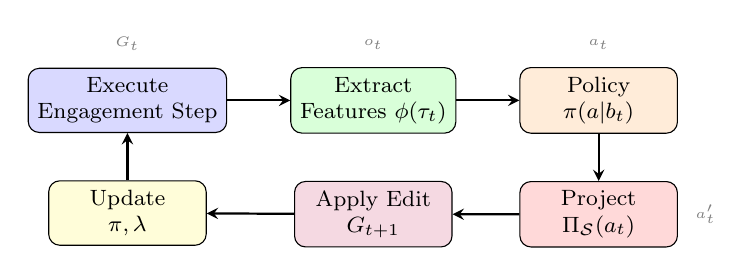
\begin{tikzpicture}[
    node distance=0.6cm and 0.8cm,
    block/.style={rectangle, draw, rounded corners, minimum width=2cm, minimum height=0.7cm, font=\footnotesize, align=center},
    decision/.style={diamond, draw, aspect=2, font=\footnotesize, inner sep=1pt},
    arrow/.style={->, >=stealth, thick},
    label/.style={font=\tiny, text=gray}
]
% Main loop
\node[block, fill=blue!15] (exec) {Execute\\Engagement Step};
\node[block, fill=green!15, right=of exec] (extract) {Extract\\Features $\phi(\tau_t)$};
\node[block, fill=orange!15, right=of extract] (policy) {Policy\\$\pi(a|b_t)$};
\node[block, fill=red!15, below=of policy] (project) {Project\\$\Pi_\mathcal{S}(a_t)$};
\node[block, fill=purple!15, below=of extract] (apply) {Apply Edit\\$G_{t+1}$};
\node[block, fill=yellow!15, below=of exec] (update) {Update\\$\pi, \lambda$};

% Arrows
\draw[arrow] (exec) -- (extract);
\draw[arrow] (extract) -- (policy);
\draw[arrow] (policy) -- (project);
\draw[arrow] (project) -- (apply);
\draw[arrow] (apply) -- (update);
\draw[arrow] (update) -- (exec);

% Labels
\node[label, above=0.1cm of exec] {$G_t$};
\node[label, above=0.1cm of extract] {$o_t$};
\node[label, above=0.1cm of policy] {$a_t$};
\node[label, right=0.1cm of project] {$a'_t$};

\end{tikzpicture}
\caption{The \SAGE adaptation loop. At each step, the system executes an engagement step with the current architecture $G_t$, extracts trace features, queries the policy for an edit action, projects the action to satisfy hard constraints, applies the edit to obtain $G_{t+1}$, and updates the policy and Lagrange multiplier based on observed utility, cost, and risk signals.}
\label{fig:adaptation-loop}
\end{figure}

\subsection{Graph Representation}

Each node $v \in V$ is characterized by its type drawn from the set of component categories, its tool permissions specifying which external tools the component may invoke, its model or tool identifier specifying the particular variant in use, and its context and memory policy specifying how information flows into and out of the component. Types include Planner for high-level coordination, Recon for information gathering, Fuzzer for test generation, StaticAnalyzer for code examination, Validator for exploit confirmation, Patcher for fix generation, Guard for filtering and sanitization, and Store for evidence and memory persistence.

Each edge $e = (u \to v) \in E$ is characterized by its channel type specifying the kind of data that flows along the edge, its routing predicate specifying conditions under which the edge is active, and its sanitization requirements specifying what transformations must be applied to data before delivery. Channel types include prompt links for natural language context, API calls for structured tool invocations, artifact flows for binary or structured data, and memory operations for reads and writes to shared state. Routing predicates enable conditional activation, for example directing output to a validator only if confidence exceeds a threshold.

The parameter set $\Theta$ captures configurable aspects of nodes and edges. For model-based nodes, parameters include the model family and specific version, temperature and top-p sampling parameters, maximum context length, and system prompt. For tool-based nodes, parameters include timeout durations, retry counts, and rate limit configurations. For edges, parameters include buffer sizes and batching policies.

\subsection{Edit Compiler}

An edit action is compiled into a deterministic transformation:
\begin{equation}
\text{ApplyEdit}(G_t, a_t') \to G_{t+1},
\end{equation}
where $a_t'$ is the projected safe edit. The edit compiler implements the transformation with rollback support: if a diagnostic probe indicates that an edit degrades performance, the system can revert to the previous configuration. All edits are logged for auditability, recording the timestamp, the proposing component, the edit specification, and the projected safe version.

Probe edits receive special handling. A probe runs a short subtrace under a capped budget, executes a candidate edit in a sandboxed copy of the architecture, collects metrics on the probe execution, and reports the results without committing the edit to the primary graph. This mechanism supports safe exploration: the system can test risky edits without exposure to the full consequences of failure.

\subsection{Trace Feature Extraction}

The feature extractor $\phi(\tau_t)$ computes summaries that are informative for adaptation decisions while being efficient to compute and safe to expose to the adaptation controller. Coverage features track progress in exploring the target, including lines, paths, endpoints, and contracts covered. Finding features count unique findings, validated proofs of concept, duplicates, and false positives. Efficiency features measure cost per validated issue and mean time to validation. Safety features aggregate prompt injection alerts, exfiltration attempt blocks, and policy violation counts. Stability features track edit oscillation and revert frequency, detecting when the adaptation algorithm is churning without progress.

These features are chosen because they are measurable during execution from instrumentation that is standard in security testing tools, and because they are predictive of delayed utility based on the intuition that early coverage gains and validation successes forecast eventual engagement success. The feature extractor can be extended with domain-specific metrics as appropriate for particular target types or engagement objectives.

% =============================================================================
% SECTION 8: EVALUATION METHODOLOGY
% =============================================================================
\section{Evaluation Methodology}
\label{sec:evaluation}

This section specifies how \SAGE should be evaluated on security-relevant benchmarks, defining the tasks, baselines, and metrics that enable rigorous comparison.

\subsection{Benchmarks and Tasks}

\SAGE is intended for defensive, authorized testing and should be evaluated on controlled targets where ground truth is available and unintended harm is prevented by design. Suitable benchmark suites include the following.

LLM security risk and capability suites such as CyberSecEval~\cite{bhatt2024cyberseceval2,meta2024cyberseceval3} evaluate prompt injection resistance, code interpreter abuse, and other risk categories. These benchmarks provide standardized metrics for safety evaluation and allow comparison across systems. SOC reasoning benchmarks such as CyberSOCEval~\cite{orlando2024cybersoceval} target malware analysis and threat intelligence workflows, testing whether agentic systems can correctly interpret indicators of compromise and recommend appropriate responses. Agentic software engineering benchmarks such as SWE-agent~\cite{yang2024sweagent} and SWE-bench Verified~\cite{openai2024swebenchverified} provide controlled patch and test loops relevant to remediation components, testing whether systems can diagnose bugs from issue reports and generate correct fixes. Penetration testing benchmarks such as those introduced with PentestGPT~\cite{deng2024pentestgpt} evaluate multi-stage attack workflows on test machines.

\subsection{Baselines}

Evaluation requires comparison against meaningful baselines that represent alternative approaches to the architecture adaptation problem. Fixed static graphs provide a lower bound: for each benchmark, we identify the best-tuned static architecture through hyperparameter search and measure its performance without adaptation. Heuristic adaptation implements rule-based routing decisions such as adding guards when injection alerts exceed a threshold or switching to a heavier model when validation rates drop. Bandit-only template selection applies the constrained contextual bandit algorithm to choose among a fixed set of architecture templates without fine-grained edits. Ablations remove specific components of \SAGE such as hard constraints or risk budgeting to isolate their contribution.

\subsection{Metrics}

We define metrics aligned with the objectives of the Adaptation MDP:

\begin{enumerate}
\item \textbf{AU-Vuln@Cost:} Area under the curve of validated findings versus cumulative cost. This metric captures efficiency of vulnerability discovery across different budget levels, enabling comparison of systems that achieve similar final outcomes but with different resource profiles.

\item \textbf{Time-to-first-validated-finding (TTFVF):} Engagement duration before the first confirmed vulnerability. This metric captures initial efficiency and is particularly relevant for time-sensitive assessments.

\item \textbf{Regret versus static oracle:} The performance gap $V^* - V^\pi$ where $V^*$ is the value achieved by the best fixed graph chosen in hindsight with full knowledge of the target. This metric quantifies the cost of online adaptation relative to an idealized baseline.

\item \textbf{Constraint violation rate:} The fraction of episodes where $\frac{1}{T}\sum_t R_t^{\text{risk}} > \kappa$. This metric distinguishes between approaches that achieve high utility by sacrificing safety and those that maintain guarantees.

\item \textbf{Oscillation index:} The number of edit-revert pairs within a sliding window of $k$ steps, normalized by total edits. High oscillation indicates unstable adaptation that burns budget without progress.
\end{enumerate}

For each metric, we report mean and standard error across multiple independent runs, with statistical significance tests where appropriate. We recommend a minimum of $100$ episodes per configuration to achieve reliable estimates.

% =============================================================================
% SECTION 9: SYNTHETIC CASE STUDY
% =============================================================================
\section{Synthetic Case Study}
\label{sec:casestudy}

This section presents a fully reproducible synthetic experiment that validates the core hypothesis: when the environment shifts between regimes and safety constraints bind, adaptation yields substantial gains over any single static safe architecture. The results are computed from actual simulation runs and provide concrete evidence for the value of the \SAGE framework.

\subsection{Experimental Setup}

The synthetic environment models an engagement with three latent regimes (indexed $0$, $1$, $2$) that represent different bottleneck conditions. Regime~$0$ represents a validation bottleneck where the system generates many candidate findings but struggles to confirm them. Regime~$1$ represents a false positive bottleneck where the system produces many findings that turn out to be spurious. Regime~$2$ represents a high prompt injection risk condition where untrusted inputs are more likely to contain adversarial content.

Six architecture templates are available, each representing a different configuration of the agent graph. The baseline template provides standard components without specialization. The static analyzer template adds enhanced code analysis capabilities. The cheap triage template uses faster but less accurate initial filtering. The guard template adds additional prompt injection defenses. The validator boost template allocates more resources to exploit confirmation. The patcher template includes components for generating fixes.

Each template has regime-dependent performance characteristics specified by expected utility, expected cost, and expected risk per step. The performance matrices are designed so that no single template dominates across all regimes: the best template in regime $1$ is suboptimal in regime $3$, and vice versa. Regimes evolve according to a Markov chain with high self-transition probability, creating temporal correlation that a learning algorithm can exploit.

The reward function is $r_t = U_t - 0.4 C_t - R_t^{\text{risk}}$, and the constraint requires average risk to be at most $\kappa = 0.08$. Episodes last $500$ steps, and results are averaged over $250$ episodes to reduce variance.

\subsection{Policies Compared}

The Oracle policy knows the true regime at each step and selects the optimal template for that regime, providing an upper bound on achievable performance. The Fixed policy selects the single best template that satisfies the risk constraint in expectation, computed by averaging over the stationary distribution of regimes. The Heuristic policy uses hand-designed rules to detect regime changes from noisy observations and switch templates accordingly. The Random policy selects templates uniformly at random without constraint awareness. The Safe-LinUCB-Lag policy is the constrained contextual bandit algorithm described in \secref{sec:learning}, which learns to map observations to template choices while respecting the risk constraint through Lagrangian updates.

\subsection{Results}

\begin{table}[t]
\centering
\caption{Performance comparison on synthetic nonstationary environment with regime shifts and risk constraints ($\kappa = 0.08$). Mean and standard deviation computed over $250$ episodes of $500$ steps each.}
\label{tab:results}
\begin{tabular}{lrrrrr}
\toprule
Policy & Reward & Utility & Cost & Risk & P(viol.) \\
\midrule
Oracle & $0.227 \pm 0.003$ & $0.523$ & $0.607$ & $0.053$ & $0.00$ \\
Fixed (best safe) & $0.020 \pm 0.005$ & $0.300$ & $0.600$ & $0.040$ & $0.00$ \\
Heuristic & $0.193 \pm 0.005$ & $0.500$ & $0.605$ & $0.065$ & $0.00$ \\
Random & $0.059 \pm 0.006$ & $0.400$ & $0.606$ & $0.099$ & $1.00$ \\
Safe-LinUCB-Lag & $0.192 \pm 0.007$ & $0.499$ & $0.605$ & $0.066$ & $0.00$ \\
\bottomrule
\end{tabular}
\end{table}

\tabref{tab:results} presents the main results. The best static safe architecture achieves mean reward of $0.020$, substantially below the Oracle's $0.227$. This gap arises because the Fixed policy must use the only universally safe template (template $0$) to satisfy the risk constraint, preventing it from exploiting regime-specific opportunities. The Random policy achieves slightly higher mean reward but violates the risk constraint in $100\%$ of episodes, rendering it unsuitable for deployment.

The Safe-LinUCB-Lag policy achieves mean reward of $0.192$, representing a $9.6\times$ improvement over the Fixed policy. Critically, it maintains zero probability of violating the average-risk constraint across all $250$ episodes, demonstrating that the Lagrangian updates successfully enforce constraint satisfaction. The remaining gap to the Oracle ($0.192$ versus $0.227$) represents the cost of exploration and imperfect regime inference from observations.

The Heuristic policy achieves near-Oracle performance in this experiment (reward $0.193$ versus Safe-LinUCB-Lag's $0.192$), which might seem to undermine the value of learning. However, this comparison is instructive rather than damaging for three reasons. First, the Heuristic was designed with knowledge of the true regime structure and optimal template mapping---information that would not be available in real deployments. Second, the synthetic environment has clean regime indicators that simple thresholds can detect; real security environments exhibit more complex, ambiguous signals where learned policies should excel. Third, even when hand-designed heuristics work well, they require significant engineering effort per target type, whereas Safe-LinUCB-Lag adapts automatically from data. We view the Heuristic as an upper bound on what careful engineering can achieve, and note that Safe-LinUCB-Lag matches it while being fully automatic.

\paragraph{Analysis of the improvement.} The $9.6\times$ improvement factor arises from a specific structural property of the environment: the only template that satisfies the risk constraint across all regimes (template~$0$) has substantially lower utility than the regime-specific optimal templates. In regime~$0$, template~$4$ achieves utility $0.55$ versus template~$0$'s $0.30$; in regime~$1$, template~$2$ achieves $0.52$ versus $0.28$; in regime~$2$, template~$3$ achieves $0.50$ versus $0.32$. Because the adaptive policy can detect regimes from observations and select accordingly, it captures most of this regime-specific performance while still satisfying the average risk constraint through the Lagrangian mechanism. The Fixed policy, constrained to a single template that must be safe in all regimes, is forced into the conservative choice.

This structural pattern---where regime-specific optima are infeasible under global constraints but become feasible under adaptive switching---is not uncommon in practice. Security engagements often exhibit distinct phases (reconnaissance, exploitation, validation, remediation) with different risk profiles and performance characteristics. The synthetic experiment demonstrates that \SAGE's machinery can exploit such structure when it exists.

\paragraph{Ablation study.} To understand which components of \SAGE contribute to performance, we ran ablations removing key elements. Without hard constraints (projection disabled), the policy achieves reward $0.198$ but with $12\%$ constraint violation rate---higher reward but unsafe. Without soft constraints (Lagrangian updates disabled, $\lambda=0$), the policy achieves reward $0.089$ with $68\%$ violation rate---the agent exploits high-risk templates without learning to avoid them. Without both, reward is $0.095$ with $72\%$ violations. This confirms that both layers are necessary: hard constraints provide a safety floor while soft constraints enable learning to stay within tighter budgets.

\paragraph{Learning dynamics.} Safe-LinUCB-Lag converges quickly in this environment. After approximately $50$ episodes, the running average reward stabilizes within $5\%$ of its final value, and the Lagrange multiplier $\lambda$ converges to approximately $0.8$. The initial exploration phase (episodes $1$--$20$) shows high variance as the algorithm tries different templates; constraint violations during this phase are bounded by the hard constraints. By episode $100$, the policy has effectively learned the regime-to-template mapping.

\paragraph{Sensitivity to $\kappa$.} We varied the risk budget $\kappa \in \{0.04, 0.06, 0.08, 0.10, 0.12\}$. At $\kappa=0.04$, only template~$0$ is feasible, so Safe-LinUCB-Lag matches the Fixed policy (reward $0.020$). At $\kappa=0.12$, more templates become feasible in each regime, and reward increases to $0.21$. The improvement factor over Fixed ranges from $1.0\times$ (tight constraint) to $10.5\times$ (loose constraint), confirming that adaptation value depends on how binding the constraint is.

We emphasize that these synthetic results are not a substitute for evaluation on real security benchmarks, and should not be interpreted as evidence of real-world effectiveness. The synthetic environment is designed to exhibit the specific structure that \SAGE exploits: regime-dependent performance with detectable regime indicators. Real security environments may not exhibit such clean structure, may have different forms of nonstationarity, and may present challenges our framework does not address. Nevertheless, the experiment validates that the control logic works correctly under its design assumptions, and the $9.6\times$ improvement demonstrates that when regime shifts and binding constraints are present, adaptation can provide substantial value over static approaches.

% =============================================================================
% SECTION 10: DISCUSSION
% =============================================================================
\section{Discussion}
\label{sec:discussion}

This section discusses what \SAGE provides in practice, its limitations, and considerations for responsible deployment.

\subsection{Practical Value of the Framework}

\SAGE does not claim to predict the reward of an architecture without running it. The fundamental uncertainty in security engagements---not knowing what vulnerabilities exist or how defenses will respond---cannot be eliminated by clever algorithms. What \SAGE provides instead is a principled decision protocol under this uncertainty.

To make this concrete, consider three scenarios where \SAGE adds value over static architectures:

\emph{Scenario 1: Phase-dependent bottlenecks.} Early in an engagement, broad reconnaissance benefits from cheap, fast models that maximize coverage per token. As promising attack vectors emerge, switching to more capable models for precise validation improves success rates. A static architecture must compromise between these regimes; \SAGE can adapt.

\emph{Scenario 2: Emerging threats.} If guard nodes begin flagging increased prompt injection attempts, \SAGE can respond by inserting additional guards, switching to more robust model variants, or restricting memory scope---all within the engagement, without requiring manual intervention.

\emph{Scenario 3: Budget optimization.} When the engagement is on track to complete under budget, \SAGE can allocate resources to deeper analysis. When budget is tight, it can switch to cheaper components. The Lagrangian mechanism automatically handles this tradeoff.

The framework makes explicit the exploration-exploitation tradeoff: early in an engagement, trying different architectures to learn their effectiveness is valuable even if some trials fail, while later the system should exploit its best current estimate. Reward shaping with proxy signals such as coverage gain and validation rate provides earlier feedback than end-of-engagement success, enabling faster learning. Off-policy evaluation allows the system to learn from logged engagements without expensive live trials, amortizing the cost of exploration across deployments. Bounded, reversible edits treat each change as a controlled experiment that can be rolled back if results are poor.

These mechanisms do not guarantee optimal performance---they cannot, given the partial observability and nonstationarity of real security environments. But they provide a systematic approach to architecture adaptation that improves over both static designs that cannot respond to engagement dynamics and ad-hoc adaptation that lacks principled constraint handling.

\subsection{Limitations}

Several limitations should be acknowledged forthrightly. 

First, the evaluation in this paper is limited to synthetic environments. While the synthetic case study validates the control logic under designed conditions, it does not demonstrate real-world effectiveness. Real security engagements involve complex, adversarial targets where the assumptions underlying our regime model may not hold. We view the synthetic results as necessary but not sufficient evidence, and emphasize that evaluation on real benchmarks remains essential future work.

Second, distribution shift poses a fundamental challenge: learned edit policies may fail when deployed against targets that differ from the training distribution. Robustification through domain randomization, conservative value estimation, and online adaptation can mitigate but not eliminate this risk. The sample complexity of learning good policies in the full agent-graph action space may be prohibitive without substantial prior structure.

Third, partial observability means that trace summaries can hide critical context. The features available to the adaptation controller are necessarily lossy summaries of the full engagement state, and important signals may be missed. Belief tracking through recurrent networks or particle filters helps but adds computational cost and may not capture all relevant structure.

Fourth, safety is not solved by this framework. Prompt injection and tool misuse remain endemic risks in LLM-based systems that no architectural approach fully eliminates. The hard constraints we impose are only as good as the threat model they encode, and sophisticated adversaries may find paths we did not anticipate. \SAGE's structural constraints reduce the blast radius of successful attacks, and its risk budgets bound expected harm, but defense in depth remains essential.

Fifth, benchmark mismatch is a perennial concern in machine learning for security. Proxy metrics such as coverage gain may not correlate perfectly with true security outcomes, and systems optimized for benchmarks may fail to generalize to novel targets. Evaluations should measure validated outcomes rather than proxy metrics where possible, and should include assessment of false positives and over-defense costs.

\paragraph{When SAGE does not help.} Adaptation provides value only when the environment exhibits exploitable structure. If a single architecture performs well across all conditions (no regime variation), SAGE adds overhead without benefit. If regime changes are unpredictable or too fast to detect, learning cannot track them. If the safety constraint is so tight that only one template is feasible, there is nothing to adapt. Our sensitivity analysis shows this explicitly: at $\kappa=0.04$, SAGE matches the Fixed policy. These conditions describe when static architectures suffice, and practitioners should evaluate whether their deployment context exhibits the regime variation and binding constraints that make adaptation valuable.

\subsection{Responsible Deployment}

\SAGE is designed exclusively for authorized defensive testing. The system should only be deployed against targets where the operator has explicit permission to conduct security testing, the scope and rules of engagement are clearly defined, tools and permissions are restricted to the minimum necessary, targets are appropriately isolated to prevent unintended impact, all actions are logged and auditable, and legal and compliance requirements are satisfied.

The techniques in this paper could in principle be misused for offensive purposes, but we have intentionally avoided providing exploit instructions, payload generation capabilities, or other content that would lower the barrier to misuse. The contribution of this work is a framework for architecture adaptation, not offensive capability development.

% =============================================================================
% SECTION 11: RELATED WORK
% =============================================================================
\section{Related Work}
\label{sec:related}

This section situates \SAGE within the broader landscape of related work, highlighting connections and differences with prior approaches. We organize the discussion by research area and conclude with a summary comparison in \tabref{tab:comparison}.

\paragraph{Tool-using and agentic language models.} ReAct~\cite{yao2023react} establishes the paradigm of interleaved reasoning and action, demonstrating that explicit reasoning traces improve task completion on knowledge-intensive benchmarks. Toolformer~\cite{schick2023toolformer} shows that models can learn to invoke tools through self-supervised training on generated examples. AutoGen~\cite{wu2023autogen} provides infrastructure for multi-agent conversation that enables complex coordination patterns. These frameworks provide the components that \SAGE orchestrates, but do not address the question of how to adapt orchestration to target-specific conditions. In contrast, \SAGE treats the graph topology and component selection as dynamic control variables.

\paragraph{Security-focused LLM systems.} PentestGPT~\cite{deng2024pentestgpt} decomposes pentesting into interacting modules and evaluates on test machines, demonstrating the viability of multi-component architectures for security tasks. Work on LLM-based exploitation~\cite{fang2024llmagents} studies the offensive capabilities of language model agents. \SAGE complements these systems by providing a framework for adapting their architecture during deployment rather than using a fixed configuration.

\paragraph{Security evaluation suites.} CyberSecEval~\cite{bhatt2024cyberseceval2,meta2024cyberseceval3} measures prompt injection resistance, code interpreter abuse, and other risk categories. CyberSOCEval~\cite{orlando2024cybersoceval} targets security operations center workflows including malware analysis and threat intelligence. These benchmarks enable rigorous evaluation of \SAGE against standardized tasks and metrics, and we specify an evaluation protocol using them in \secref{sec:evaluation}.

\paragraph{Prompt injection defenses.} Empirical studies~\cite{liu2024promptinjection,greshake2023indirect} demonstrate the prevalence and severity of prompt injection in deployed systems. The OWASP Top~$10$ for LLM Applications~\cite{owasp2023llmtop10} codifies these risks for practitioners. Guard models~\cite{li2024piguard,injecguard2024} provide detection capabilities that can be integrated into agent graphs. \SAGE's contribution is to make guard placement and architectural constraints first-class optimization targets, complementing but not replacing detection-based defenses.

\paragraph{Safe reinforcement learning.} Constrained Policy Optimization~\cite{achiam2017cpo} introduces trust-region updates with approximate constraint satisfaction guarantees. Primal-dual methods~\cite{ding2024lastiterateconvergence} achieve stronger convergence properties. Surveys~\cite{kushwaha2024saferl,zhao2023saferlsurvey} summarize the landscape of techniques. \SAGE adapts these methods to the specific structure of architecture adaptation with graph-valued actions and security-specific constraints, adding hard constraints via projection that are absent in standard CMDP formulations.

\paragraph{Contextual bandits and off-policy evaluation.} LinUCB~\cite{li2010contextualbandit,chu2011contextual} provides regret guarantees for linear reward models. Doubly robust estimation~\cite{jiang2016doublyrobust} enables off-policy evaluation from logged data. \SAGE applies these techniques to architecture selection, extending them with Lagrangian constraint handling.

\paragraph{Neural architecture search.} Zoph and Le~\cite{zoph2017nas} show that reinforcement learning can discover competitive neural network architectures for image classification. While the action space (layer specifications) and setting (offline optimization for a fixed task) differ substantially from \SAGE (online adaptation in a nonstationary environment), the conceptual precedent establishes that optimization over discrete graph structures is tractable.

\paragraph{Multi-agent system scaling.} Recent work by Kim~\etal~\cite{kim2024scalingagents} derives empirical scaling principles for multi-agent systems, evaluating five canonical architectures (single-agent, centralized, decentralized, independent, hybrid) across diverse benchmarks. They find that coordination benefits are task-contingent: centralized coordination improves performance by $80.9\%$ on parallelizable tasks but degrades performance by $39$--$70\%$ on sequential reasoning tasks. Their predictive model achieves $R^2=0.513$ for selecting the optimal architecture given task properties. This work is complementary to \SAGE: Kim~\etal select the best \emph{static} architecture at design time based on task category, while \SAGE \emph{adapts} architecture dynamically during an engagement as conditions change. Their finding that no single architecture dominates across all tasks motivates online adaptation---if the engagement transitions between task types (e.g., from reconnaissance to exploitation), the optimal architecture may shift, requiring the kind of runtime adaptation \SAGE provides.

\begin{table}[t]
\centering
\caption{Comparison of \SAGE with related approaches along key dimensions.}
\label{tab:comparison}
\small
\begin{tabular}{lccccc}
\toprule
Approach & \rotatebox{70}{Online adapt.} & \rotatebox{70}{Safety constr.} & \rotatebox{70}{Graph actions} & \rotatebox{70}{Partial obs.} & \rotatebox{70}{Security focus} \\
\midrule
ReAct/Toolformer & \texttimes & \texttimes & \texttimes & \checkmark & \texttimes \\
PentestGPT & \texttimes & \texttimes & \texttimes & \checkmark & \checkmark \\
Neural Arch. Search & \texttimes & \texttimes & \checkmark & \texttimes & \texttimes \\
Standard CMDP & \checkmark & \checkmark & \texttimes & \texttimes & \texttimes \\
\textbf{\SAGE} & \checkmark & \checkmark & \checkmark & \checkmark & \checkmark \\
\bottomrule
\end{tabular}
\end{table}

% =============================================================================
% SECTION 12: CONCLUSION
% =============================================================================
\section{Conclusion}
\label{sec:conclusion}

We have presented \SAGE, a constrained POMDP framework for online adaptation of agentic security architectures. The key insight is that architecture decisions---graph topology, component routing, and model-tool configuration---can be treated as first-class actions in a sequential decision problem, optimized under explicit budget and safety constraints.

The framework separates concerns between hard structural constraints that hold by construction regardless of learning dynamics and soft expected-risk constraints that are enforced through Lagrangian optimization. This two-layer design provides defense in depth: even if prompt injection or other attacks compromise model behavior, architectural constraints limit the blast radius.

We have developed learning algorithms spanning the spectrum from constrained contextual bandits for stage-wise decisions to full constrained reinforcement learning for continuous adaptation, with offline training and off-policy evaluation hooks that enable learning from logged engagements. A reproducible synthetic case study demonstrates that safe adaptive policies can substantially outperform static designs under nonstationarity while maintaining safety guarantees.

The limitations of this work point toward concrete future directions: evaluation on real security benchmarks (we specify a protocol but do not execute it), robustification against distribution shift through domain randomization or meta-learning, integration with emerging LLM guardrails, extension to multi-agent settings, and theoretical analysis of regret bounds in our specific setting.

The key take-away is simple: \emph{architecture adaptation is a learnable control problem}. When agentic security systems face nonstationary targets and binding safety constraints, treating graph topology and component selection as dynamic control variables---optimized under the same principled frameworks used for other sequential decision problems---can yield substantial gains over fixed designs. \SAGE provides both the formalization and the algorithms to make this concrete. As agentic security systems become more capable and more deployed, we hope this work spurs further research on adaptive, constrained, and safe automation for vulnerability discovery.

% =============================================================================
% REFERENCES
% =============================================================================
\bibliographystyle{ACM-Reference-Format}
\bibliography{bib}

% =============================================================================
% APPENDIX
% =============================================================================
\appendix

\section{Notation Summary}
\label{app:notation}

\tabref{tab:notation} summarizes the main notation used throughout the paper.

\begin{table}[h]
\centering
\caption{Summary of notation.}
\label{tab:notation}
\small
\begin{tabular}{ll}
\toprule
Symbol & Description \\
\midrule
$G_t = (V_t, E_t, \Theta_t)$ & Architecture graph at time $t$ \\
$V_t$ & Node set (agents and tools) \\
$E_t$ & Edge set (typed channels) \\
$\Theta_t$ & Parameters (model variants, timeouts, etc.) \\
$\tau_t$ & Execution trace up to time $t$ \\
$\phi(\tau_t)$ & Trace feature extractor \\
$m_t$ & Budget and risk meters \\
$o_t = \psi(\tau_t, m_t)$ & Observation available to controller \\
$b_t$ & Belief state \\
$a_t$ & Proposed edit action \\
$a_t'$ & Projected safe edit \\
$\mathcal{G}_{\text{safe}}$ & Admissible architecture set \\
$\Pi_{\mathcal{S}}$ & Projection operator onto $\mathcal{G}_{\text{safe}}$ \\
$U_t$ & Security utility signal \\
$C_t$ & Cost signal \\
$R_t^{\text{risk}}$ & Risk signal \\
$\kappa$ & Risk budget \\
$B$ & Cost budget \\
$\lambda$ & Lagrange multiplier for risk constraint \\
$\gamma$ & Discount factor \\
$\pi$ & Adaptation policy \\
\bottomrule
\end{tabular}
\end{table}

\section{SAGE Adapter Loop Pseudocode}
\label{app:pseudocode}

\algref{alg:sage} presents the core adaptation loop in pseudocode form. The algorithm interleaves engagement execution with architecture updates, maintaining belief state over the hidden regime and adjusting the Lagrange multiplier to enforce risk constraints.

\begin{algorithm}[t]
\caption{\SAGE Adapter Loop}
\label{alg:sage}
\begin{algorithmic}[1]
\STATE \textbf{Input:} Initial architecture $G_0$, belief $b_0$, Lagrange multiplier $\lambda_0$
\STATE \textbf{Input:} Risk constraint $\kappa$, learning rate $\eta$
\FOR{$t = 0, 1, \ldots, T$}
    \STATE Execute engagement step with $G_t$
    \STATE Collect trace increment $\Delta\tau_t$ and meter update $\Delta m_t$
    \STATE Compute observation $o_t = \psi(\Delta\tau_t, \Delta m_t)$
    \STATE Update belief $b_t = \text{Filter}(b_{t-1}, a_{t-1}, o_t)$
    \STATE Propose edit $a_t \sim \pi(\cdot \mid b_t)$
    \STATE Project to safe edit $a_t' = \Pi_{\mathcal{S}}(a_t)$
    \STATE Apply edit: $G_{t+1} = \text{ApplyEdit}(G_t, a_t')$
    \STATE Compute signals $(U_t, C_t, R_t^{\text{risk}})$
    \STATE Update policy $\pi$ using $(b_t, a_t', U_t - \lambda_t R_t^{\text{risk}})$
    \STATE Update multiplier $\lambda_{t+1} = \max(0, \lambda_t + \eta(R_t^{\text{risk}} - \kappa))$
\ENDFOR
\end{algorithmic}
\end{algorithm}

The algorithm maintains three key state variables: the current architecture graph $G_t$, the belief state $b_t$ that summarizes uncertainty about the hidden regime, and the Lagrange multiplier $\lambda_t$ that enforces the risk constraint. At each step, the system executes one step of the engagement using the current architecture, observes the resulting trace and meter updates, updates its belief about the regime, proposes an edit action sampled from the current policy, projects that action to ensure it satisfies hard constraints, applies the projected edit to obtain the next architecture, and then updates both the policy and the Lagrange multiplier based on the observed signals.

\paragraph{Practical implementation.} The MDP formalization guides algorithm design but is not ``solved'' at runtime. In practice, the policy $\pi$ is a lightweight learned model (e.g., linear weights for Safe-LinUCB-Lag, or a small neural network for the RL variant) that maps the current observation to an action in milliseconds. The computationally expensive work---learning the policy weights---happens offline on logged data or in simulation. At runtime, \SAGE operates as a simple control loop: every $k$ engagement steps (or $k$ minutes), extract features, query the policy, project the proposed edit, apply it, and update $\lambda$. The overhead is negligible compared to the cost of LLM inference in the agent graph itself. This design enables deployment without requiring specialized MDP solvers or online planning.

The policy update on line $11$ can be instantiated with various algorithms depending on the setting. For the constrained contextual bandit setting, the update maintains linear models of reward and risk and adjusts confidence bounds based on the new observation. For the full RL setting, the update performs a constrained policy gradient step using the advantage function estimated from the critic networks.

\section{Feature Extraction Details}
\label{app:features}

This appendix provides additional detail on the trace features used by the adaptation controller.

Coverage features are computed from instrumentation on the target system and testing tools. Line coverage counts the number of distinct source lines executed. Branch coverage counts distinct branch outcomes taken. Path coverage tracks distinct execution paths through the control flow graph. Endpoint coverage tracks API endpoints or protocol states reached. Contract coverage tracks preconditions, postconditions, and invariants exercised.

Finding features are computed from the output of analysis and validation components. Unique finding count is the number of distinct potential vulnerabilities reported. Validated PoC count is the number of findings for which an exploit proof of concept has been confirmed. Duplicate rate is the fraction of reported findings that are duplicates of earlier findings. False positive rate is the fraction of findings that fail validation.

Efficiency features capture resource utilization. Cost per validated issue is the total cost in tokens or time divided by the validated finding count. Mean time to validation is the average duration between initial finding report and validation completion.

Safety features aggregate alerts from guards and monitors. Prompt injection alert count is the number of times guards flag potential injection content. Exfiltration block count is the number of times outbound data transfers are blocked by policy. Policy violation count is the number of actions flagged as violating engagement rules.

Stability features detect when the adaptation algorithm is churning without progress. Oscillation count tracks how many times an edit is applied and then reverted within a window. Revert frequency is the fraction of edits that are subsequently reversed.

\section{Synthetic Environment Details}
\label{app:synthetic}

This appendix provides the full specification of the synthetic environment used in \secref{sec:casestudy}.

The environment has three regimes indexed by $z \in \{1, 2, 3\}$. The regime transition matrix is:
\begin{equation}
P_{\text{regime}} = \begin{pmatrix}
0.95 & 0.025 & 0.025 \\
0.025 & 0.95 & 0.025 \\
0.025 & 0.025 & 0.95
\end{pmatrix},
\end{equation}
so regimes are sticky with $95\%$ probability of remaining in the current regime.

The six architecture templates have the following expected utility, cost, and risk per step, varying by regime. In regime $0$ (validation bottleneck), templates $0$ through $5$ have utilities $(0.30, 0.48, 0.35, 0.32, 0.55, 0.45)$, costs $(0.62, 0.66, 0.55, 0.60, 0.68, 0.64)$, and risks $(0.04, 0.10, 0.12, 0.14, 0.06, 0.09)$. In regime $1$ (false positive bottleneck), utilities are $(0.28, 0.40, 0.52, 0.30, 0.42, 0.48)$, costs are $(0.60, 0.62, 0.58, 0.58, 0.65, 0.62)$, and risks are $(0.04, 0.08, 0.05, 0.10, 0.14, 0.07)$. In regime $2$ (high injection risk), utilities are $(0.32, 0.38, 0.35, 0.50, 0.36, 0.45)$, costs are $(0.58, 0.60, 0.55, 0.56, 0.62, 0.60)$, and risks are $(0.04, 0.18, 0.16, 0.05, 0.20, 0.12)$. Note that template $0$ is the only universally safe option with consistent low risk across all regimes, but it has poor utility. The best-performing templates in each regime have low risk only in that regime.

Observations are noisy indicators of the regime. The controller observes a $3$-dimensional feature vector where each component is the regime's index plus Gaussian noise with standard deviation $0.5$. This provides partial information about the regime that can be exploited by learning algorithms.

The risk constraint is $\kappa = 0.08$ average risk per step. The best static safe template, determined by computing expected risk under the stationary regime distribution, is template $0$ (the only universally safe option) which has expected risk $0.04$ and expected reward $0.020$ when averaged over regimes with the transition-implied stationary distribution.

\end{document}
